\documentclass{beamer}
\usepackage[utf8]{inputenc}
\usepackage[english]{babel}
\usepackage[style=british]{csquotes}
\usepackage{verbatim}
\usepackage{listings}
\usepackage{graphicx}
\usepackage{amsmath}
\usepackage{calc}
\usepackage{array}
\usepackage{xcolor}
\usepackage{pgf}
\usepackage{tikz}
\usetikzlibrary{arrows,calc,intersections,through,decorations.pathmorphing,backgrounds,positioning,fit,shapes}
\usepackage[T1]{fontenc}
\usepackage{minted}
\usepackage{ulem}
\usepackage{hyperref}
\usepackage{booktabs}
\usetheme{Boadilla}
\AtBeginSection[]
%{
%  \begin{frame}<beamer>
%      \frametitle{Syllabus}
%      {\scriptsize\tableofcontents[currentsection,hideothersubsections]
%      }
%    \end{frame}
%}

\tikzset{
  invisible/.style={opacity=0},
  visible on/.style={alt=#1{}{invisible}},
  alt/.code args={<#1>#2#3}{%
    \alt<#1>{\pgfkeysalso{#2}}{\pgfkeysalso{#3}} % \pgfkeysalso doesn't change the path
  },
}

\definecolor{dgreen}{rgb}{0.,0.6,0.}
\definecolor{RawSienna}{cmyk}{0,0.72,1,0.45}

\title{kubernetes}
\author{Scality}
\date{\today}


\begin{document}

\maketitle{}

\section{History}

\begin{frame}
\frametitle{Can you guess ?}
\centering
\vfill
around 10 Billions dollars
\vfill
\visible<2->{yearly Google infrastructure cost}
\end{frame}

\begin{frame}
  \frametitle{Once upon a time (at Google{\tiny ™®©}, Inc.)}
  \begin{center}
  \href{https://research.google.com/pubs/pub44843.html}
       {https://research.google.com/pubs/pub44843.html}
  \vfill
  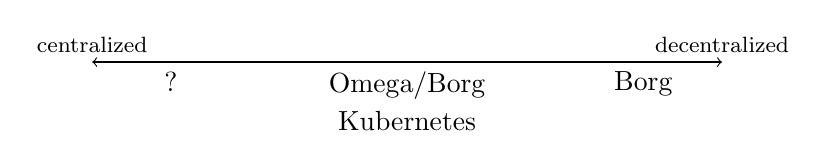
\begin{tikzpicture}
    \draw[<->] (-4,0) -- (4,0)
    node[at start, above] {\footnotesize{centralized}}
    node[at end, above] {\footnotesize{decentralized}}
    node[very near start, below] {?}
    node[very near end, below, visible on=<2->] {Borg}
    node[midway, below,visible on=<3->] {Omega/Borg}
    node[midway, below,yshift=-0.5cm, visible on=<4->] {Kubernetes};
  \end{tikzpicture}
  \end{center}
\end{frame}

\begin{frame}
  \frametitle{Docker}
  \begin{itemize}
    \item container "Isolated" by filesystem, network and process from host
    \item Image hub to fetch image
    \item filesystem modification temporary by design
    \item mount "external" filesystem to store data (aka volume)
  \end{itemize}
\end{frame}


\begin{frame}
  \frametitle{Pods}
  \begin{columns}
  \begin{column}{0.5\textwidth}
    \begin{center}
    \begin{tikzpicture}
      \node[draw, label=above:\scriptsize{\it{simple-pod.yaml}}] (pod) {
        \begin{minipage}{0.6\textwidth}
          \inputminted[fontsize=\scriptsize]{yaml}{resources/simple-pod.yaml}
        \end{minipage}
      };
      \node[draw,below=0.8cm of pod] (kubectl) {kubectl};
      \node[below=1.4cm of kubectl]  (kubernetes) {
        \pgftext{\includegraphics[height=2cm]{img/kubernetes}}
      };
      \draw[->] (pod) -- (kubectl);
      \draw[->] (kubectl) to ($ (kubernetes) + (0,0.7cm) $);
    \end{tikzpicture}
    \end{center}
  \end{column}
  \begin{column}{0.5\textwidth}
    \begin{itemize}
      \item<1-> Minimum schedulable unit
      \item<2-> Multiple containers. Often a main process with \textit{sidecars}
        like watchdogs, conf-managers, monitoring adapters
      \item<3-> With common network (distinct or shared with the host)
    \end{itemize}
  \end{column}
  \end{columns}
\end{frame}

\begin{frame}
  \frametitle{Namespaces}
  \enquote{
    Namespaces provide a scope for names. Names of resources need to be unique within a namespace, but not across namespaces.
    \newline
    Namespaces are a way to divide cluster resources between multiple users.
  }
  \newline

  \hfill Kubernetes Documentation

  \vfill
  \scriptsize{
    \begin{block}{3 "default" namespace}
    \begin{itemize}
      \item kube-system
      \item default
      \item kube-public
    \end{itemize}
    \end{block}
  }
\end{frame}

\begin{frame}
  \frametitle{Architecture}
  \begin{center}
  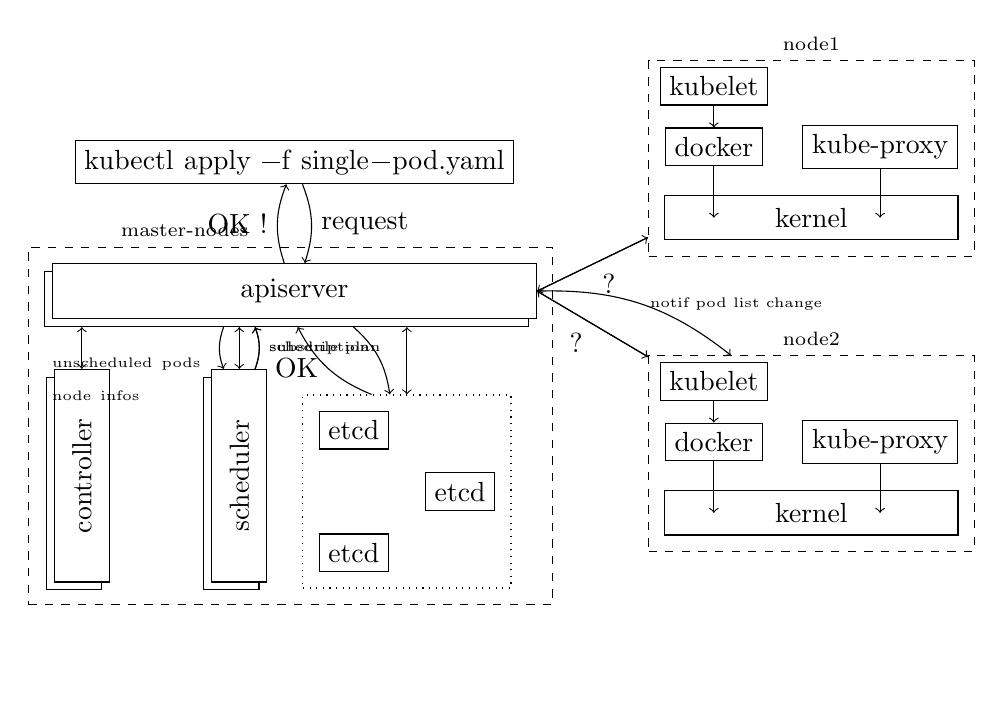
\begin{tikzpicture}
    \def\nbetcd{3}
    \def\nbapiserver{2}
    \def\nbscheduler{2}
    \def\nbcontroller{2}
    \def\nbnode{2}
    \edef\alletcd{}
    \foreach \i in {1,...,\nbetcd}{
      \node[draw] at ($ (360/\nbetcd * \i:0.9) $) (etcd\i) {etcd};
      \xdef\alletcd{(etcd\i) \alletcd}
    }
    \node[draw,dotted, fit=\alletcd, inner sep=2mm] (etcd) {};

    % Scheduler
    \visible<10->{
      \foreach \i in {1,...,\nbscheduler}{
        \node[draw,
              rotate fit=90,
              % Warning all anchor are rotated
              left=of etcd,
              fill=white,
              fit=(etcd.north west) (etcd.south west),
              minimum height=0.7cm,
              xshift=\i mm,
              yshift=-\i mm] (scheduler\i) {};
      }
      \node[draw=none, align=center,rotate=90] at (scheduler\nbscheduler) {scheduler};
    }

    % Controller
    \visible<15->{
      \foreach \i in {1,...,\nbcontroller}{
        \node[draw,
              rotate fit=90,
              % Warning all anchor are rotated
              left=3cm of scheduler1,
              fill=white,
              fit=(etcd.north west) (etcd.south west),
              minimum height=0.7cm,
              xshift=\i mm,
              yshift=-\i mm] (controller\i) {};
      }
      \node[align=center,rotate=90] at (controller\nbcontroller) {controller};
    }
    % Apiserver
    \visible<2->{
      \foreach \i in {1,...,\nbapiserver}{
        \node[draw,
              above=of etcd,
              fill=white,
              fit=(scheduler1.north east) (controller1.north east) (etcd.north east),
              minimum height=0.7cm,
              xshift=\i mm,
              yshift=\i mm,
          ] (apiserver\i) {};
      }
      \node[align=center] at (apiserver\nbapiserver) {apiserver};
      \draw[<->] (etcd.north) -- (etcd.north|-apiserver1.south);
    }

    % Request flow
    \visible<3-6>{
      \node[draw,above=of apiserver\nbapiserver] (kubectl)
            {\lstinline{kubectl apply -f single-pod.yaml}};
      \draw[->,bend left=20] (kubectl) to
            node[midway,
                 anchor=west] {request}
            (apiserver\nbapiserver);
    }

    \visible<4-6>{
      \draw[->] (apiserver1) to [bend left=20] (etcd.100);
    }
    \visible<5-6>{
      \draw[->,bend left=20] (etcd.110) to
        node[midway,anchor=east] {OK}
        (apiserver1);

    }
    \visible<6>{
      \draw[->,bend left=20] (apiserver\nbapiserver) to
            node[midway,
                 anchor=east] {OK !}
            (kubectl);
    }

    % Nodes
    \visible<8->{
      \node[above right=3cm of apiserver\nbapiserver] (kubelet1) {};
      \foreach \i in {1,...,\nbnode}{
        \node[draw] (kubelet-box\i) at (kubelet\i) {kubelet};
        \node[draw,below=0.4cm of kubelet\i] (docker\i) {docker};
        \node[draw,right=0.5cm of docker\i] (kube-proxy\i) {kube-proxy};
        \node[draw,below=0.9cm of docker\i,
              fit=(docker\i) (kube-proxy\i),
              inner sep=0mm] (kernel\i) {};
        \node[align=center] at (kernel\i) {kernel};
        \draw[->] (kubelet-box\i) -- (docker\i);
        \draw[->] (docker\i) -- (docker\i|-kernel\i);
        \draw[->] (kube-proxy\i) -- (kube-proxy\i |- kernel\i);
        \node[draw,
              dashed,
              fit=(kubelet\i) (docker\i) (kube-proxy\i) (kernel\i),
              inner sep=2mm,
              label={\scriptsize{node\i}}]  (node\i) {};
        \draw[<->] (node\i) -- (apiserver\nbapiserver.east);

        \pgfmathtruncatemacro\nextnode{\i+1}
        \node[draw=none, below=3.5cm of kubelet\i] (kubelet\nextnode) {};
      }
    }

    % Action on node
    \visible<9>{
      \foreach \i in {1,...,\nbnode}{
        \draw (node\i) to [draw=none,edge label=?] (apiserver\nbapiserver.east);
      }
    }

    %Scheduler action
    \visible<10->{
      \draw[<->] (scheduler\nbscheduler.east) -- (scheduler\nbscheduler.east|-apiserver1.south);
    }
    \visible<11-12>{
      \draw[->,bend right=20] ($(scheduler\nbscheduler.east) + (2mm,0)$)
             to node[midway,anchor=west]{\tiny{subscription}}
            ($(scheduler\nbscheduler.east|-apiserver1.south) + (2mm,0)$);

    }
    \visible<12>{
      \draw[->,bend right=20] ($(scheduler\nbscheduler.east|-apiserver1.south) + (-2mm,0)$)
            to node[midway,anchor=north east,text width=2cm]{\tiny{unscheduled pods \\ node infos}}
            ($(scheduler\nbscheduler.east) + (-2mm,0)$);
    }
    \visible<13>{
      \draw[->,bend right=20] ($(scheduler\nbscheduler.east) + (2mm,0)$)
             to node[midway,anchor=west]{\tiny{schedule plan}}
            ($(scheduler\nbscheduler.east|-apiserver1.south) + (2mm,0)$);
    }
    \visible<14>{
        \draw[->,bend left=20] (apiserver\nbapiserver.east)
             to node[midway,anchor=west]{\tiny{notif pod list change}}
             (node2);
    }
    %Controller
    \visible<15->{
      \draw[<->] (controller\nbscheduler.east) -- (controller\nbscheduler.east|-apiserver1.south);
    }

    \visible<16->{
      \node[draw,
            dashed,
            fit=(etcd) (apiserver1) (apiserver\nbapiserver),
            inner sep=2mm,
            label={[visible on=<5->,anchor=south west]above left:\scriptsize{master-nodes}}] (masternodes) {};
    }

  \end{tikzpicture}
  \end{center}
\end{frame}

\begin{frame}
  \frametitle{Controller-manager}
  \begin{columns}
  \begin{column}{0.3\textwidth}
    \textit{Deployment/replicaset}
    \inputminted[fontsize=\tiny,frame=single]{yaml}{resources/deployment.yaml}
  \end{column}
  \begin{column}{0.39\textwidth}
    \textit{Statefulset}
    \inputminted[fontsize=\tiny,frame=single]{yaml}{resources/statefulset.yaml}
  \end{column}
  \begin{column}{0.3\textwidth}
    \textit{Daemonset (<1.12)}
    \inputminted[fontsize=\tiny,frame=single]{yaml}{resources/daemonset.yaml}
    \scriptsize{
      Spawn on each node but still honoring \textit{nodeAffinity} (like the two other kind)
    }
  \end{column}
  \end{columns}
  \begin{columns}
  \begin{column}{0.4\textwidth}
    \scriptsize{
      \begin{itemize}
        \item nginx-65d66858b-kldpd
        \item nginx-65d66858b-r4tlw
        \item nginx-65d66858b-rzbll
        \item nginx-59fc846856-lgfc7
      \end{itemize}
    }
  \end{column}
  \begin{column}{0.3\textwidth}
    \scriptsize{
      \begin{itemize}
        \item nginx-1
        \item nginx-2
        \item nginx-3
      \end{itemize}
    }
  \end{column}
  \begin{column}{0.3\textwidth}
    \scriptsize{
      \begin{itemize}
        \item nginx-node-a
        \item nginx-node-b
        \item nginx-node-d
        \item ...
      \end{itemize}
    }
  \end{column}
  \end{columns}

\end{frame}

\begin{frame}[fragile]
  \frametitle{Services}
  \begin{columns}
  \begin{column}{0.3\textwidth}
    \begin{center}
    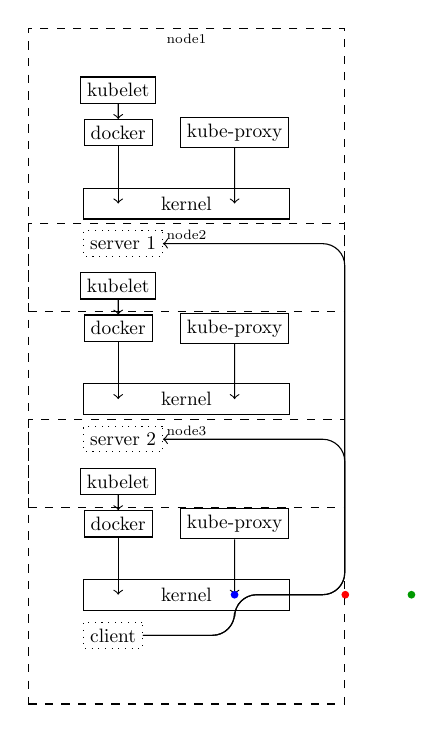
\begin{tikzpicture}[every node/.style={draw,shape=rectangle,transform shape},scale=0.7]
      \def\nbnode{3}
      \node[draw=none] (kubelet1) {};
      \foreach \i in {1,...,\nbnode}{
        \node (kubelet-box\i) at (kubelet\i) {kubelet};
        \node[below=0.4cm of kubelet\i] (docker\i) {docker};
        \node[right=0.5cm of docker\i] (kube-proxy\i) {kube-proxy};
        \node[below=0.9cm of docker\i,
              fit=(docker\i) (kube-proxy\i),
              inner sep=0mm] (kernel\i) {};
        \node[draw=none, align=center] at (kernel\i) {kernel};
        \draw[->] (kubelet-box\i) -- (docker\i);
        \draw[->] (docker\i) -- (docker\i|-kernel\i);
        \draw[->] (kube-proxy\i) -- (kube-proxy\i |- kernel\i);

        \pgfmathtruncatemacro\nextnode{\i+1}
        \node[draw=none, below=3.3cm of kubelet\i] (kubelet\nextnode) {};
      }

      \node[dotted,
            below =0.2cm of kernel1.south west,
            anchor=north west]
            (container1) {server 1};
      \node[dotted,
            below=0.2cm of kernel2.south west,
            anchor=north west]
            (container2) {server 2};
      \node[dotted,
            below=0.2cm of kernel3.south west,
            anchor=north west]
            (container3) {client};
      \foreach \i in {1,...,\nbnode}{
        \node[dashed,
              fit=(kubelet\i) (docker\i) (kube-proxy\i) (kernel\i) (container\i),
              inner sep=7mm,
              label={[anchor=north]\scriptsize{node\i}}]  (node\i) {};
      }
      \visible<2->{
        \draw[->,rounded corners=8pt]
          (container3) -| (kube-proxy2 |- kernel3.east)
          -- ($ (kernel3.east) + (1cm,0) $) |- (container1);
        \draw[->,rounded corners=8pt]
          (container3) -| (kube-proxy2 |- kernel3.east)
          -- ($ (kernel3.east) + (1cm,0) $) |- (container2);
      }
      \visible<6->{
        \fill [blue] (kube-proxy2 |- kernel3.east) circle (2pt);
        \fill [red] ($(node3.north east)!(kernel3.east)!(node3.south east)$) [label=foo] circle (2pt);
        \fill [dgreen] ($(node3.north east)!(kernel3.east)!(node3.south east) + (1.2cm, 0)$) circle (2pt);
      }
    \end{tikzpicture}
    \end{center}
  \end{column}
  \begin{column}{0.6\textwidth}
    \scriptsize{
      \visible<3->{
         \textit{service.yaml}
         \inputminted[fontsize=\scriptsize,frame=single]{yaml}{resources/service.yaml}
      }

      \begin{itemize}
        \item<4-> Fast internal loadbalancer leveraging iptables/IPVS
        \item<5-> Resolvable DNS: \\
          \scriptsize{'\lstinline{my-service.my-namespace.svc.cluster.local}'}
      \end{itemize}

      \visible<6->{
        \begin{block}{\scriptsize{Different flavour}}
          \begin{itemize}
            \item \color{blue} type=ClusterIP
            \item \color{red} type=Nodeport
            \item \color{dgreen} type=LoadBalancerIP
          \end{itemize}
         \end{block}
       }
     }
  \end{column}
  \end{columns}

\end{frame}

\section{Lego Building}

\begin{frame}{CNCF \textendash \href{https://l.cncf.io}{https://l.cncf.io}}
  \begin{figure}
        \begin{center}
            \includegraphics[width=\textwidth]{img/cncf_landscape_light.png}
        \end{center}
    \end{figure}
\end{frame}

\begin{frame}[fragile]
  \frametitle{Networking \footnotesize{(or how kubernetes is NOT doing networking)}}
  \begin{block}{Plugin contract}
    \begin{itemize}
      \item Every pod gets an unique IP
      \item Every pod IP is reachable by other pods, nodes, and master-nodes
      \item Don't conflict with Service virtualIP system (or you have to replace it)
    \end{itemize}
  \end{block}
  \scriptsize{
    \begin{table}
      \begin{tabular}{|c|c|c|c|c|c|} \hline
Provider    & OSI       & \tiny{Routable Overlay} & \tiny{Encapsulation} & \tiny{Net. Policies} & Ext. Datastore \\ \hline
Calico      & L3        & Yes(BGP)         & IPIP/No       & Yes              & Etcd (optional) \\ \hline
Flannel     & L2        & No               & Vxlan         & No               & No              \\ \hline
Canal       & L2        & No               & Vxlan         & Yes              & Etcd (optional) \\ \hline
Romana      & L3        & Yes(OSPF)        & No            & Yes              & Etcd            \\ \hline
Weave       & L2        & No               & vxlan/aws     & Yes              & No              \\ \hline
Kube-router & L3        & Yes(BGP)         & IPIP/No       & Yes              & No              \\ \hline
Cilium      & BPF/L2/L3 & No/Yes(extern)   & Vxlan         & Yes              & No              \\ \hline
      \end{tabular}
    \end{table}
  }
\end{frame}

\begin{frame}
  \frametitle{Ingress}
  \begin{columns}
  \begin{column}{0.5\textwidth}
    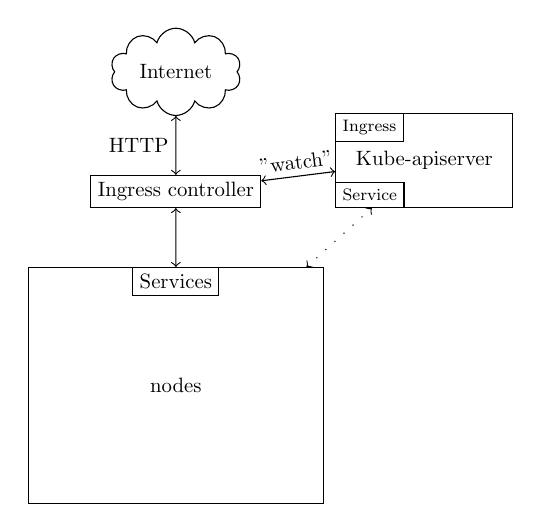
\begin{tikzpicture}[every node/.style={draw,shape=rectangle,transform shape},scale=0.75]
      \node[] (ingress) {Ingress controller};
      \node[below=of ingress, minimum height=4cm, minimum width=5cm]
        (nodes) {nodes};
      \node[below] (svc) at (nodes.north) {Services};
      \node[above=of nodes.north east, xshift=1.7cm,
          minimum height=1.6cm, minimum width=3cm] (masters) {Kube-apiserver};
      \node[below right] (ingress resource) at (masters.north west) {\footnotesize{Ingress}};
      \node[above right] (ingress resource) at (masters.south west) {\footnotesize{Service}};
      \node[shape=cloud,above=of ingress, aspect=2] (internet) {Internet};

      \draw[<->] (ingress) -- (nodes);
      \draw[<->, loosely dotted] (nodes) -- (masters);
      \draw[<->] (ingress) -- node[draw=none,above,sloped]{"watch"} (masters);
      \draw[<->] (ingress) -- node[draw=none,left,midway]{HTTP} (internet);
    \end{tikzpicture}
  \end{column}
  \begin{column}{0.5\textwidth}
    \textit{\scriptsize{ingress.yaml}}
    \inputminted[fontsize=\tiny,frame=single]{yaml}{resources/ingress.yaml}

    \scriptsize{
      \begin{block}{}
          Available controllers: \textbf{GKE}, \textbf{nginx},
            haproxy, voyager, Traefik, Kong, F5, Nginx Inc., Istio, ALB(AWS), ...

          \tiny{\textbf{(bold: officially supported by kubernetes developper)}}
      \end{block}
    }
  \end{column}
  \end{columns}
\end{frame}

\begin{frame}
  \frametitle{Helm}
  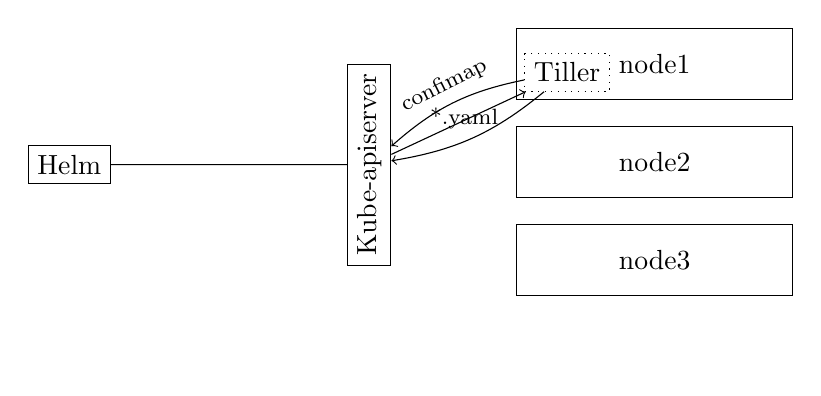
\begin{tikzpicture}
    \def\nbnode{3}
    \node[draw] (helm) {Helm};
    \node[draw,right=3cm of helm, rotate=90,anchor=north] (apiserver) {Kube-apiserver};
    \node[right=3cm of apiserver, xshift=0.5cm] (node1) {};
    \foreach \i in {1,...,\nbnode}{
      \node[draw,minimum height=0.9cm, minimum width=3.5cm] (node\i-box) at (node\i) {node\i};
      \pgfmathtruncatemacro\nextnode{\i+1}
      \node[below=1cm of node\i] (node\nextnode) {};
    }
    \node[draw,dotted,anchor=south west, xshift=1mm, yshift=1mm] (tiller) at (node1-box.south west) {Tiller};
    \visible<2-3>{
      \draw[->,rounded corners=8pt] (helm) -- (apiserver) -- (tiller);
    }
    \visible<3>{
      \draw[->,rounded corners=8pt,bend right=15] (tiller) to
        [edge node={node [sloped,above] {\footnotesize{confimap}}}]
        (apiserver);
    }
    \visible<4->{
      \draw[->,rounded corners=8pt,bend left=15] (tiller) to
        node[near start, anchor=east] {\footnotesize{*.yaml}}
        (apiserver);
    }
  \end{tikzpicture}

  \visible<5->{
    \begin{tabular}{ll}
      ~~\llap{\textbullet}~~dev:    & helm install foo -f no-autoscaling.yaml \\
      ~~\llap{\textbullet}~~staging:& helm install foo -f no-s3-mock.yaml -f staging-env.yaml \\
      ~~\llap{\textbullet}~~prod:   & helm install foo -f no-s3-mock.yaml -f production-env.yaml \\
    \end{tabular}
  }
\end{frame}

\begin{frame}
  \frametitle{prometheus}

  \begin{figure}
    \begin{center}
      \includegraphics[width=\textwidth]{img/prometheus_architecture.png}
    \end{center}
  \end{figure}
\end{frame}

\begin{frame}
  \frametitle{istio}
  \begin{figure}
    \begin{center}
      \includegraphics[width=\textwidth]{img/istio_arch.png}
    \end{center}
  \end{figure}
\end{frame}

\begin{frame}
  \frametitle{Custom Ressource Definition}
  \begin{columns}
  \begin{column}{0.6\textwidth}
    \inputminted[fontsize=\tiny,frame=single]{yaml}{resources/service-monitor.yaml}
  \end{column}
  \end{columns}
\end{frame}

\end{document}
